\subsection{Acrylglas}
\begin{tabular}{p{3.6cm}p{\textwidth-3.6cm-0.7cm}}
	\rule{0pt}{11pt}\textit{Typ}              & Lagerung und Bohrung in Acrylglas  \\ 
	\rule{0pt}{11pt}\textit{Datum}:           & 21.11.2014   \\
	\rule{0pt}{11pt}\textit{Ort}:             & Labor HSLU \\
	\rule{0pt}{11pt}\textit{Tester}:          & Matteo, Pascal\\
	\rule{0pt}{11pt}\textit{Ziel des Testes}: & Lassen sich Wälzlager in Acrylglas (PMMA) einpressen und halten sie den herrschenden Druck stand? Verhalten, Möglichkeiten von Bohrungen in $5 mm$ Acrylglas. \\
	\rule{0pt}{11pt}\textit{Aufbau / Ablauf}: & Die Bohrung ist mit einer Standbohrmaschine realisiert worden. Das Lager ist mit hilfe des Bohrkopfes der Standbohrmaschine in das Acrylglas gepresst worden.\\
	\rule{0pt}{11pt}\textit{Fazit / Verbesserungs-\newline vorschlag}: & Beim ersten Versuch sind Spannungsrisse aufgetreten (siehe Pfeil in Abbildung \ref{abb:LagerPlexiglas}). 
	Um dem entgegenzuwirken, wurde in einem zweiten Versuch die $16 mm$ Bohrung mit 
	Schleifpapier geringfügig vergrössert, damit sich das Lager leichter einpressen lässt. 
	Die Kräfte, die durch das Lager aufgenommen werden können, sind nun zwar 
	geringer, allerdings für den geplanten Einsatzbereich immer noch genügend. 
	Durch diese Methode treten auch keine Spannungsrisse mehr auf. \newline	
	Die Bohrung sollte mit einem sehr scharfen Bohrer mit stumpfem Winkel 
	gemacht werden. Weiter sollte sie gekühlt werden, um ein Durchschmelzen 
	durch die sehr dünne, noch verbleibende Restwandstärke, zu verhindern.  \\
\end{tabular}
\begin{figure}[h!]
	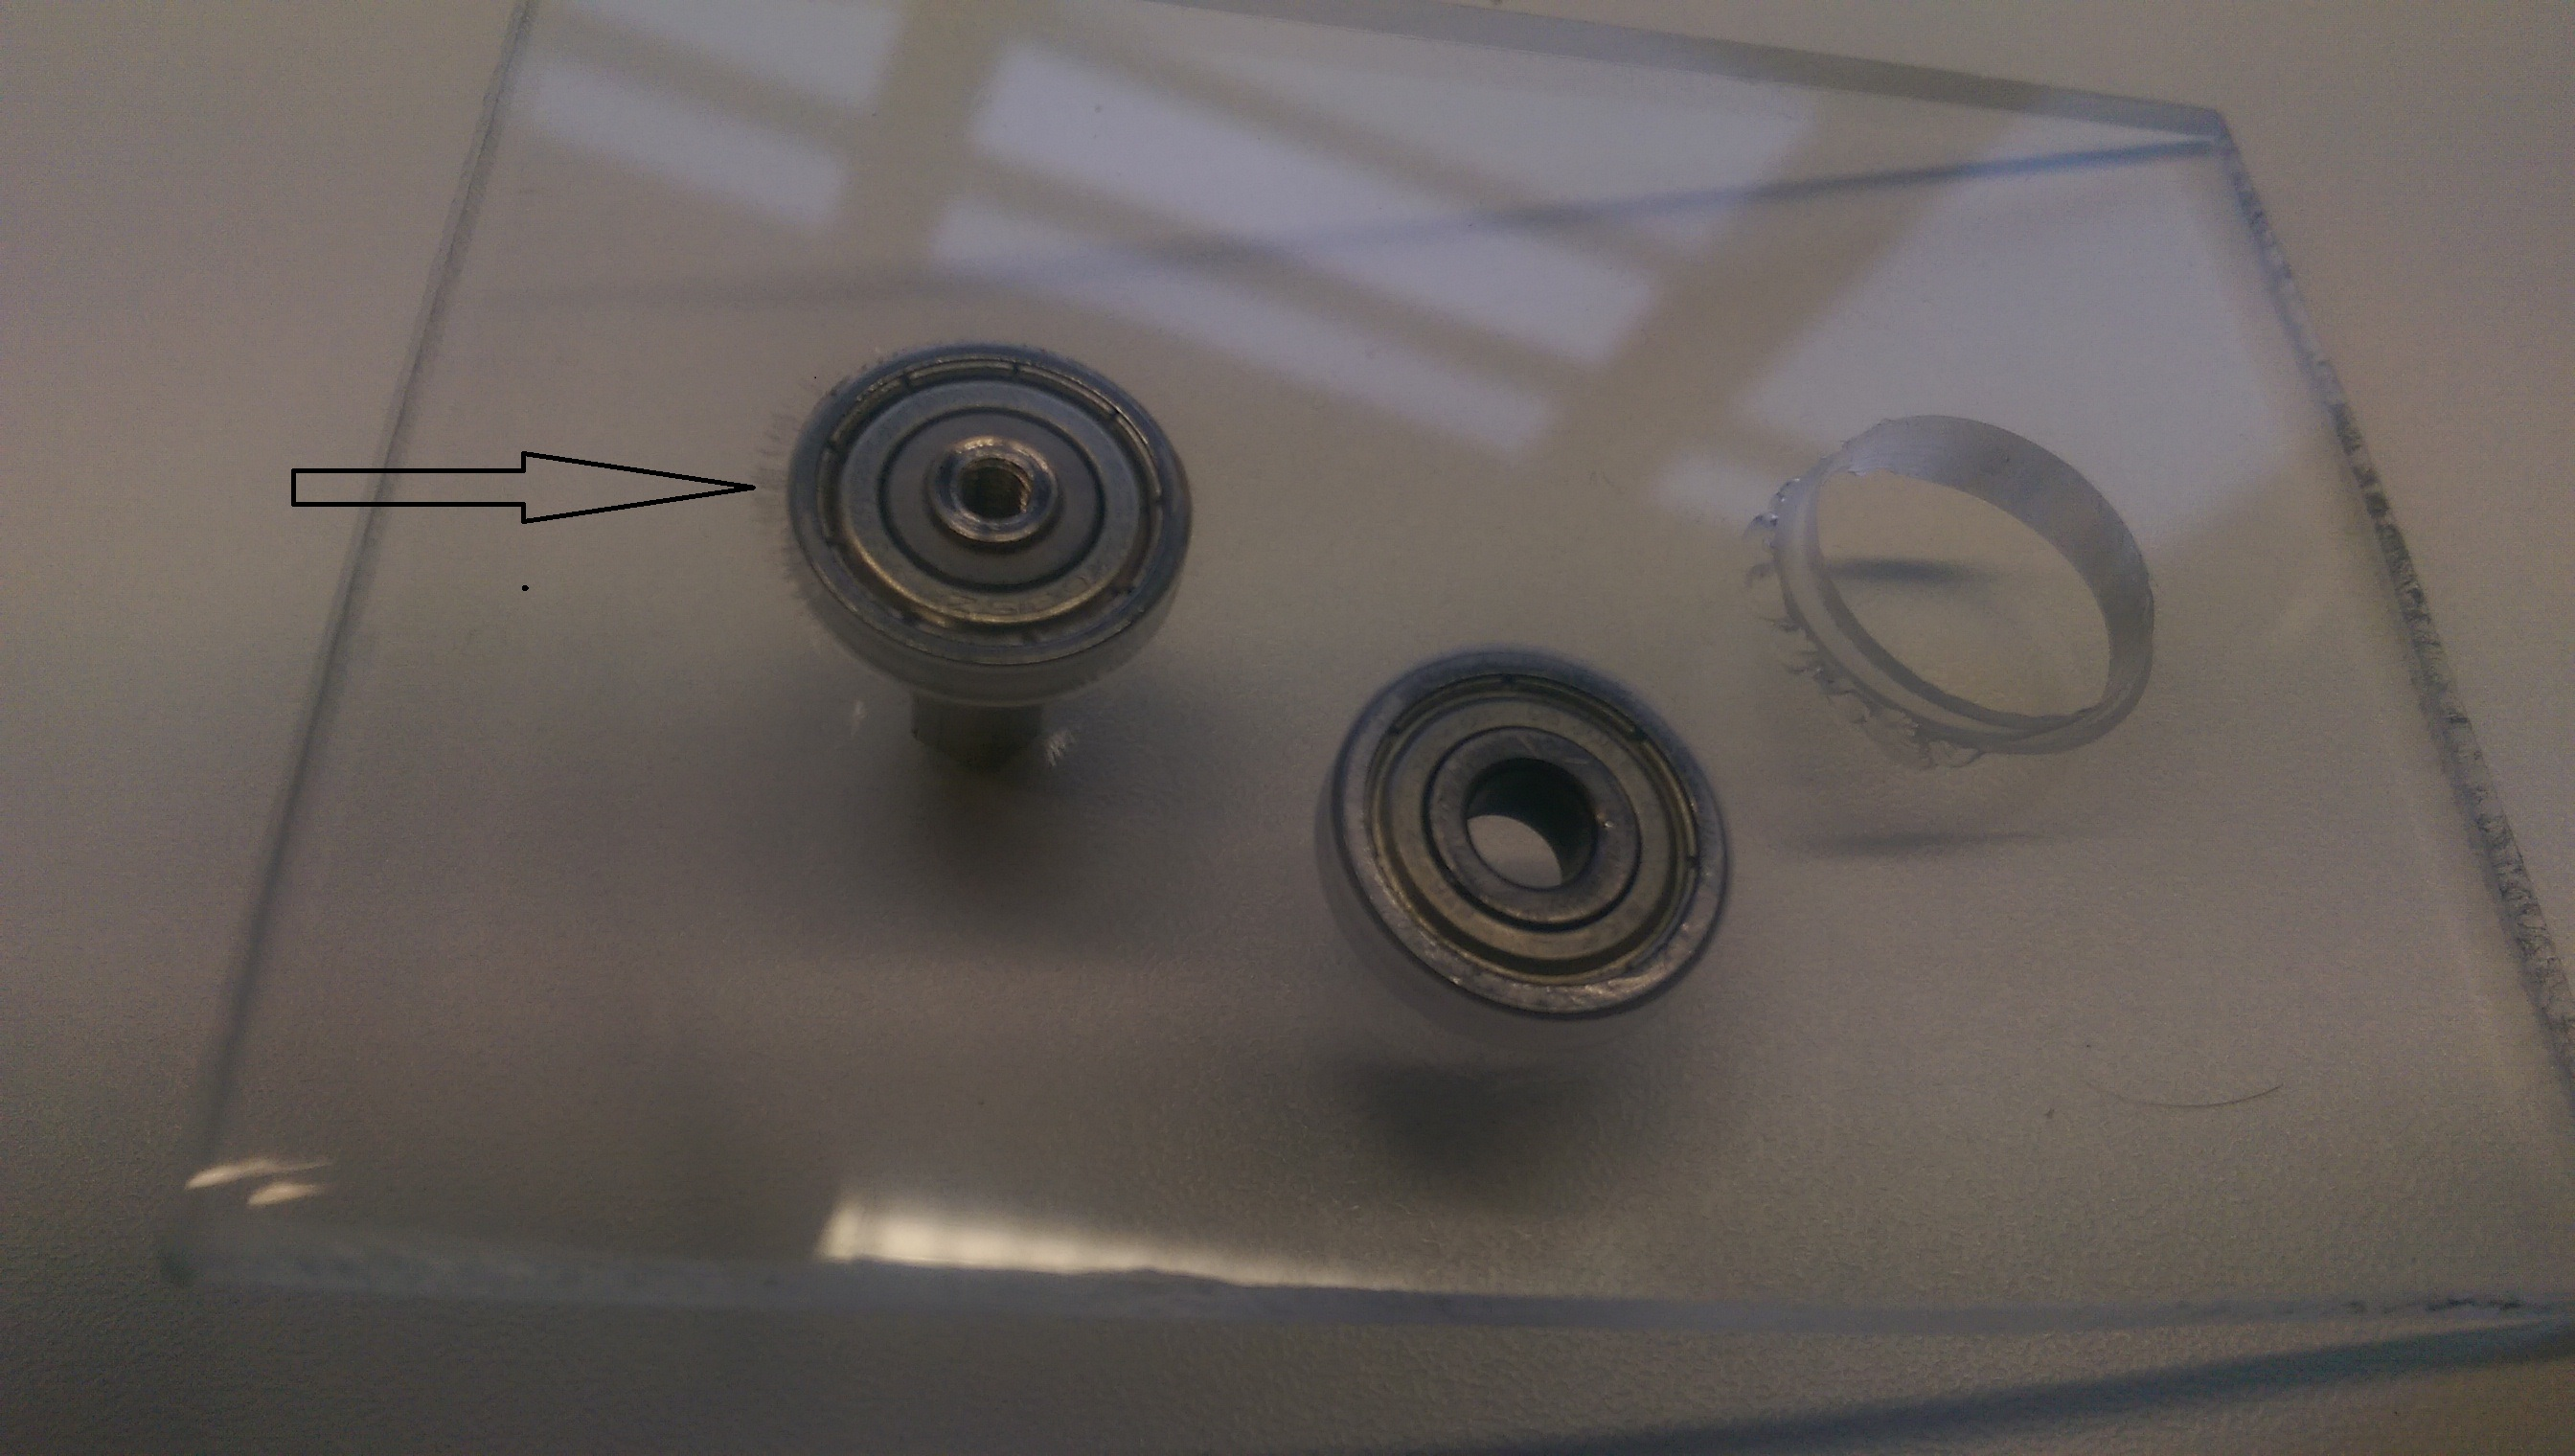
\includegraphics[width=0.9\textwidth,clip,trim=10cm 15cm 40cm 6cm]
	{Funktionstests/Bilder/LagerPlexiglas.jpg}
	\centering
	\caption{Spannungsrisse in Acrylglas-Funktionsmuster} 
	\label{abb:LagerPlexiglas}
\end{figure}